\begin{figure*}[t]
\begin{center}
\centerline{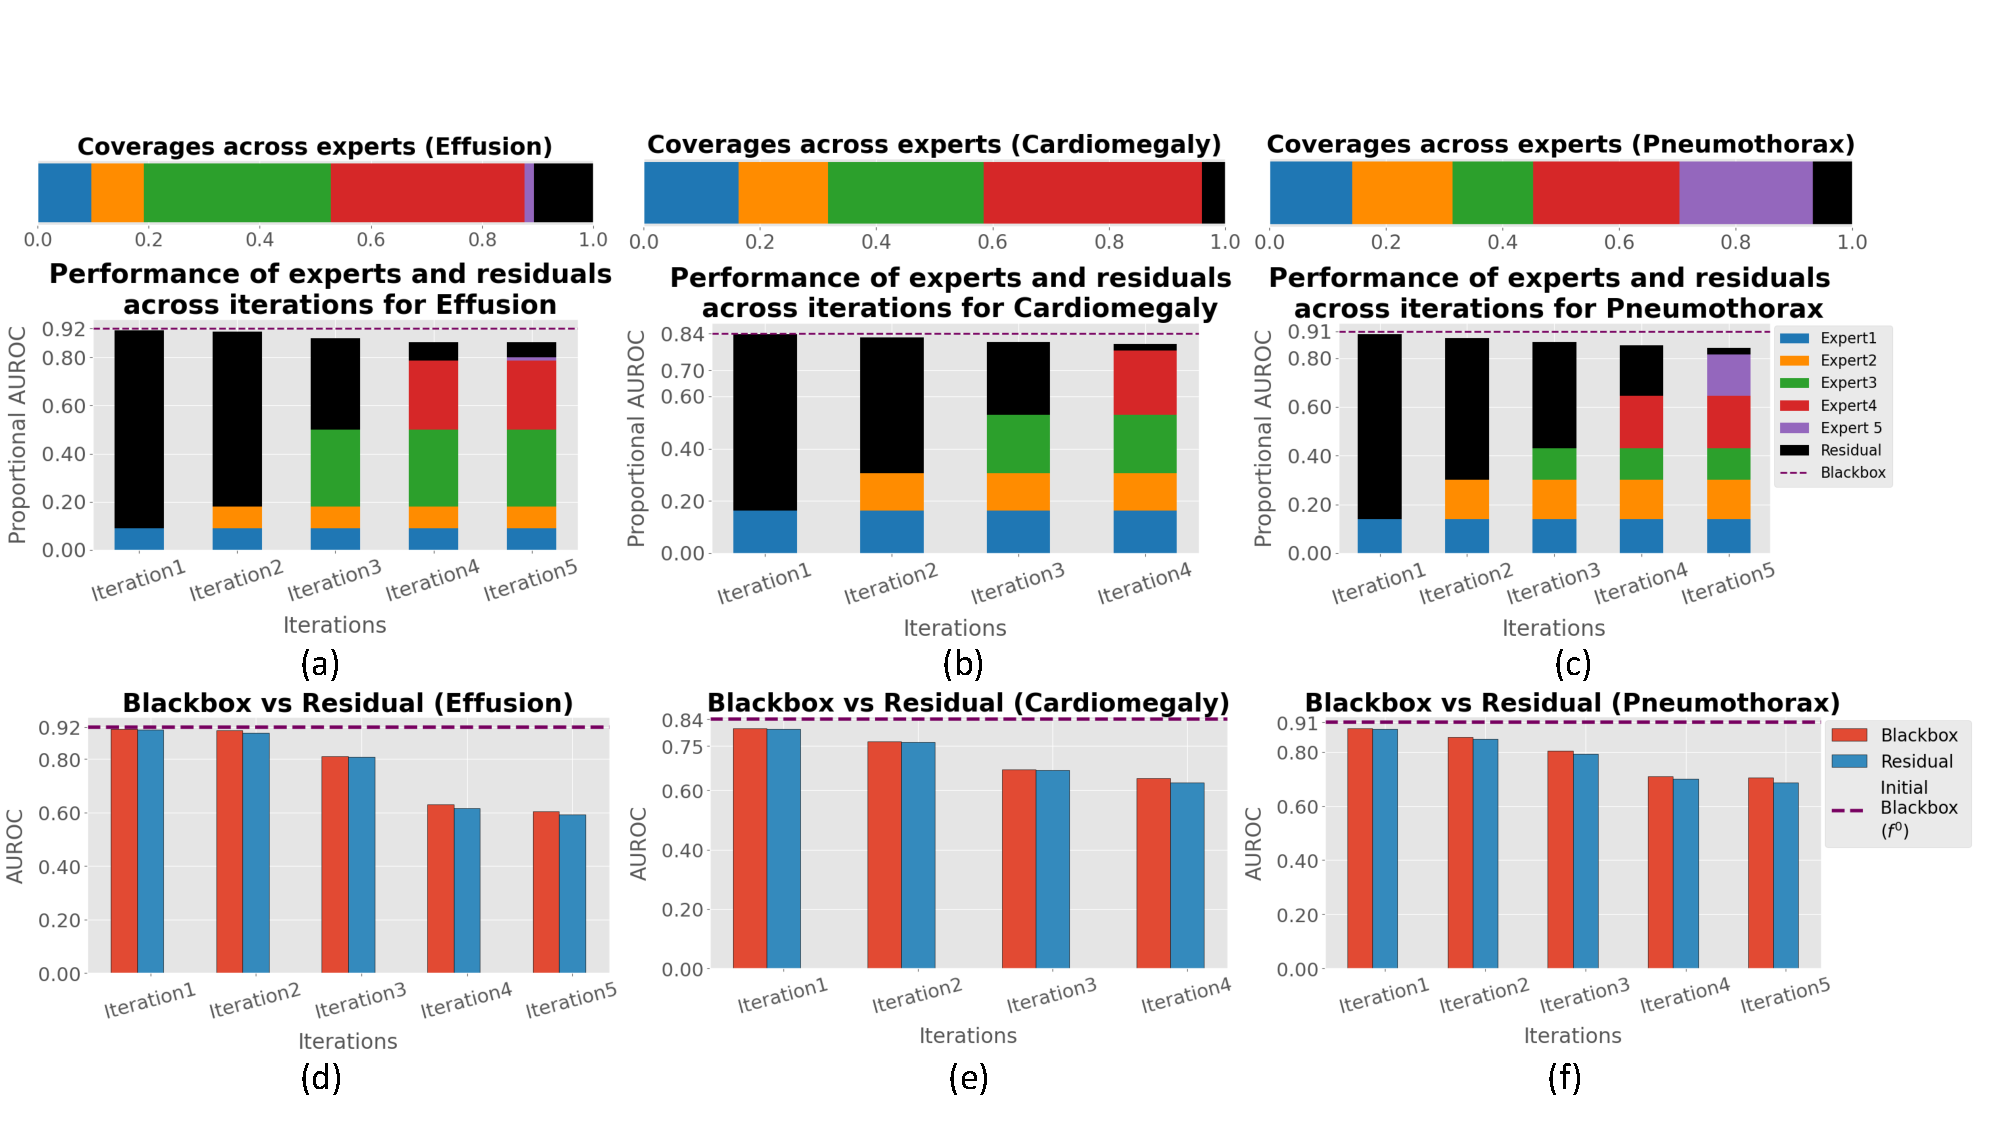
\includegraphics[width=\linewidth]{plots/main/Experts.pdf}}
\caption{Performance of experts and residuals across iterations. 
\textbf{(a-c):} Coverage and proportional AUROC of the experts and residuals.
\textbf{(d-f):} Routing the samples covered by MoIE-CXR to the initial $f^0$, we compare the performance of the residuals with $f^0$.
}
\label{fig:expert_performance_cv_vit}
\end{center}
\end{figure*}

\noindent \textbf{Identification of harder samples by successive residuals.}
Fig.~\ref{fig:expert_performance_cv_vit} (a-c) reports the proportional AUROC of the experts and the residuals per iteration. The proportional AUROC is the AUROC of that model times the empirical coverage, $\zeta^k$, the mean of the samples routed to the model by the respective selector ($\pi^k$).
According to Fig.~\ref{fig:expert_performance_cv_vit}a in iteration 1, the residual (black bar) contributes more to the proportional AUROC than the expert1 (blue bar) for effusion with both achieving a cumulative proportional AUROC~$\sim$ 0.92. All the final experts collectively extract the entire interpretable component from BB $f^0$ in the final iteration, resulting in their more significant contribution to the cumulative performance. In subsequent iterations, the proportional AUROC decreases as the experts are distilled from the BB of the previous iteration. The BB is derived from the residual that performs progressively worse with each iteration. The residual of the final iteration covers the ``hardest'' samples. Tracing these samples back to the original BB $f^0$, $f^0$ underperforms on these samples (Fig.~\ref{fig:expert_performance_cv_vit} (d-f)) as the residual.


